\documentclass[10pt]{beamer}

\usepackage[spanish, mexico]{babel}
\usepackage[utf8]{inputenc}

\usetheme[progressbar=frametitle]{metropolis}
\usepackage{appendixnumberbeamer}

\usepackage{booktabs}
\usepackage[scale=2]{ccicons}

\usepackage{tikz}
\def\checkmark{\tikz\fill[scale=0.4](0,.35) -- (.25,0) -- (1,.7) -- (.25,.15) -- cycle;}
\usepackage{pgfplots}
\usepgfplotslibrary{dateplot}

\usepackage{xspace}
\newcommand{\themename}{\textbf{\textsc{metropolis}}\xspace}

%%
\usepackage{color}
\definecolor{lstgrey}{rgb}{0.95,0.95,0.95}
\definecolor{mygreen}{RGB}{28,172,0} % color values Red, Green, Blue
\definecolor{mylilas}{RGB}{170,55,241}

\usepackage{listings}
\lstset{language=Python,
       backgroundcolor=\color{lstgrey},
       frame=single,
       basicstyle=\footnotesize\ttfamily,
       captionpos=b,
       tabsize=2,
  }

\lstset{language=Python,%
  %basicstyle=\color{red},
  breaklines=true,%
  morekeywords={python2tikz},
  keywordstyle=\color{blue},%
  morekeywords=[2]{1}, keywordstyle=[2]{\color{black}},
  identifierstyle=\color{black},%
  stringstyle=\color{mylilas},
  commentstyle=\color{mygreen},%
  showstringspaces=false,%without this there will be a symbol in the places where there is a space
  numbers=left,%
  numberstyle={\tiny \color{black}},% size of the numbers
  numbersep=9pt, % this defines how far the numbers are from the text
  emph=[1]{for,end,break},emphstyle=[1]\color{red}, %some words to emphasise
  %emph=[2]{word1,word2}, emphstyle=[2]{style},    
}
%

\lstset{language=C,
       backgroundcolor=\color{lstgrey},
       frame=single,
       basicstyle=\footnotesize\ttfamily,
       captionpos=b,
       tabsize=2,
  }

\lstset{language=C,%
  %basicstyle=\color{red},
  breaklines=true,%
  morekeywords={c2tikz},
  keywordstyle=\color{blue},%
  morekeywords=[2]{1}, keywordstyle=[2]{\color{black}},
  identifierstyle=\color{black},%
  stringstyle=\color{mylilas},
  commentstyle=\color{mygreen},%
  showstringspaces=false,%without this there will be a symbol in the places where there is a space
  numbers=left,%
  numberstyle={\tiny \color{black}},% size of the numbers
  numbersep=9pt, % this defines how far the numbers are from the text
  emph=[1]{for,end,break},emphstyle=[1]\color{red}, %some words to emphasise
  %emph=[2]{word1,word2}, emphstyle=[2]{style},    
}
%


\title{ISI437 - Inteligencia Artificial}
\subtitle{Algoritmos Genéticos}
\date{\today}
% \date{}
\author{Ing. Jose Eduardo Laruta Espejo}
\institute{Universidad La Salle - Bolivia}
% \titlegraphic{\hfill
\includegraphics[height=1.5cm]{logo.pdf}}

\begin{document}

\maketitle

\begin{frame}[allowframebreaks]{Contenido}
  \setbeamertemplate{section in toc}[sections numbered]
  \tableofcontents[]
\end{frame}

%%%

\section{Algoritmos Evolutivos}
\subsection{Introducción}
\begin{frame}
  \frametitle{Algoritmos Evolutivos}

  Los algoritmos evolutivos son un conjunto de algoritmos de optimización
  metaheurística basados en poblaciones genéricas. Los AE, utilizan mecanismos 
  inspirados por la \alert{evolución biológica} tales como reproducción, 
  mutación, recombinación y selección.
  
\end{frame}

\begin{frame}
  \frametitle{Algoritmos Evolutivos}

  En un algoritmo evolutivo, existen \textbf{soluciones candidatas} que 
  juegan el papel de individuos en una población y una \alert{función de competencia} 
  o \textit{fitness function} determina la calidad de la solución. Luego, se desarrolla
  una evolución de la población luego de la aplicación repetida de los operadores 
  anteriormente mencionados.
  
\end{frame}

\begin{frame}
  \frametitle{Algoritmos Evolutivos}

  Los algoritmos evolutivos se usan para resolver problemas de optimización y búsqueda 
  de todo tipo de manera efectiva ya que no se necesitan suposiciones sobre la calidad 
  de la solución.
  
\end{frame}

\begin{frame}
  \frametitle{Implementación}

  De una forma general, un algoritmo evolutivo sigue el siguiente esquema:
  \begin{enumerate}
    \item Generar una población de individuos aleatoriamente,
    \item Repetir lo siguiente para cada generación:
    \begin{enumerate}
      \item Evaluar la competencia (fitness) de cada individuo.
      \item Seleccionar individuos para reproducción.
      \item Generar una nueva camada de individuos.
      \item Evaluar la competendia de cada individuo.
      \item Reemplazar los individuos más débiles con los nuevos.
    \end{enumerate}
  \end{enumerate}
  
\end{frame}

\subsection{Tipos de algoritmos evolutivos}

\begin{frame}
  \frametitle{Tipos de algoritmos evolutivos}

  Existen distintos algoritmos y técnicas que siguen estos principios. 
  \begin{itemize}
    \item Algoritmos genéticos.
    \item Programación genética.
    \item Programación evolutiva.
    \item Evolución diferencial.
    \item Neuroevolución.
  \end{itemize}
\end{frame}

\section{Introducción a los algoritmos genéticos}
\begin{frame}
  \frametitle{Principio de selección natural}
  \begin{columns}
    \begin{column}{0.5\textwidth}
      \textit{Selecciona al mejor, descarta al resto.}
    \end{column}
    \begin{column}{0.5\textwidth}
      \begin{figure}[!h] 
        \centering
        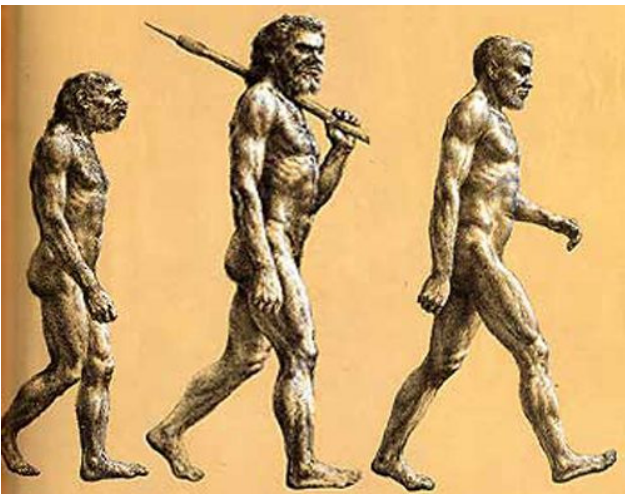
\includegraphics[width=0.9\textwidth]{img/evo}
      \end{figure}  
    \end{column}
  \end{columns}
\end{frame}

\begin{frame}
  \frametitle{Un ejemplo}
  Las jirafas tienen cuellos largos.
  \begin{columns}
    \begin{column}{0.6\textwidth}
      \begin{itemize}
        \item Las jirafas con cuellos más largos pueden alimentarse de hojas más altas.
        \item Tienen más chance de sobrevivir.
        \item Características favorables se propagan a través de las generaciones.
        \item La especie evolucionada tiene cuellos largos.
      \end{itemize}
    \end{column}
    \begin{column}{0.4\textwidth}
      \begin{figure}[!h] 
        \centering
        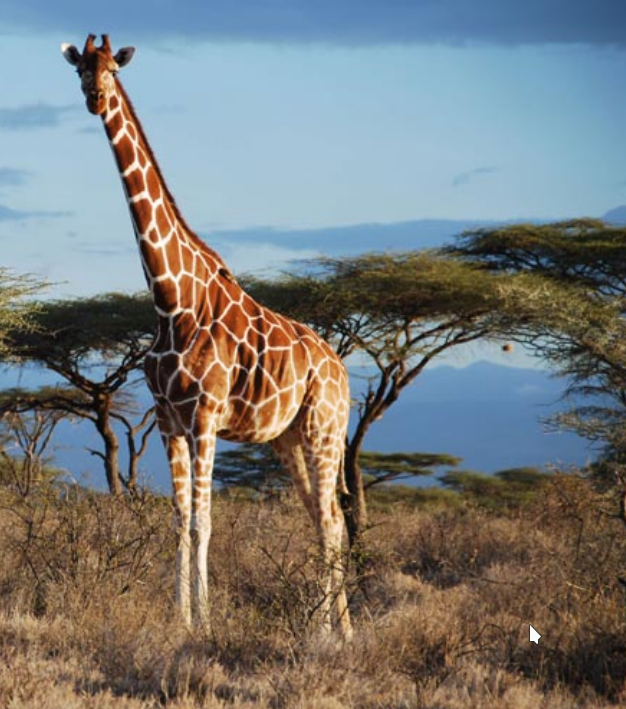
\includegraphics[width=0.9\textwidth]{img/jirafa}
      \end{figure}  
    \end{column}
  \end{columns}
\end{frame}

\begin{frame}
  \frametitle{Un ejemplo}
  Las jirafas tienen cuellos largos.
  \begin{columns}
    \begin{column}{0.6\textwidth}
        Inicialmente cuellos más largos pudieron aparecer por efectos 
        de la mutación, pero los resultados positivos se propagaron 
        en futuras generaciones
    \end{column}
    \begin{column}{0.4\textwidth}
      \begin{figure}[!h] 
        \centering
        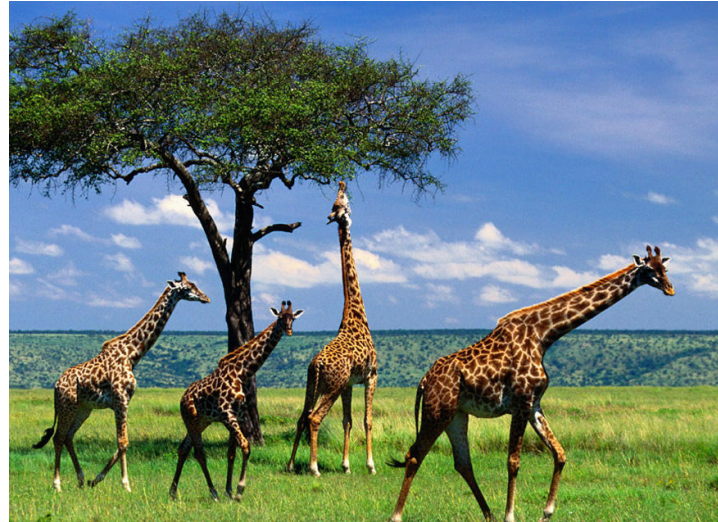
\includegraphics[width=1\textwidth]{img/jirafa2}
      \end{figure}  
    \end{column}
  \end{columns}
\end{frame}

\begin{frame}
  \frametitle{Evolución de las especies}
  \begin{figure}[!h] 
    \centering
    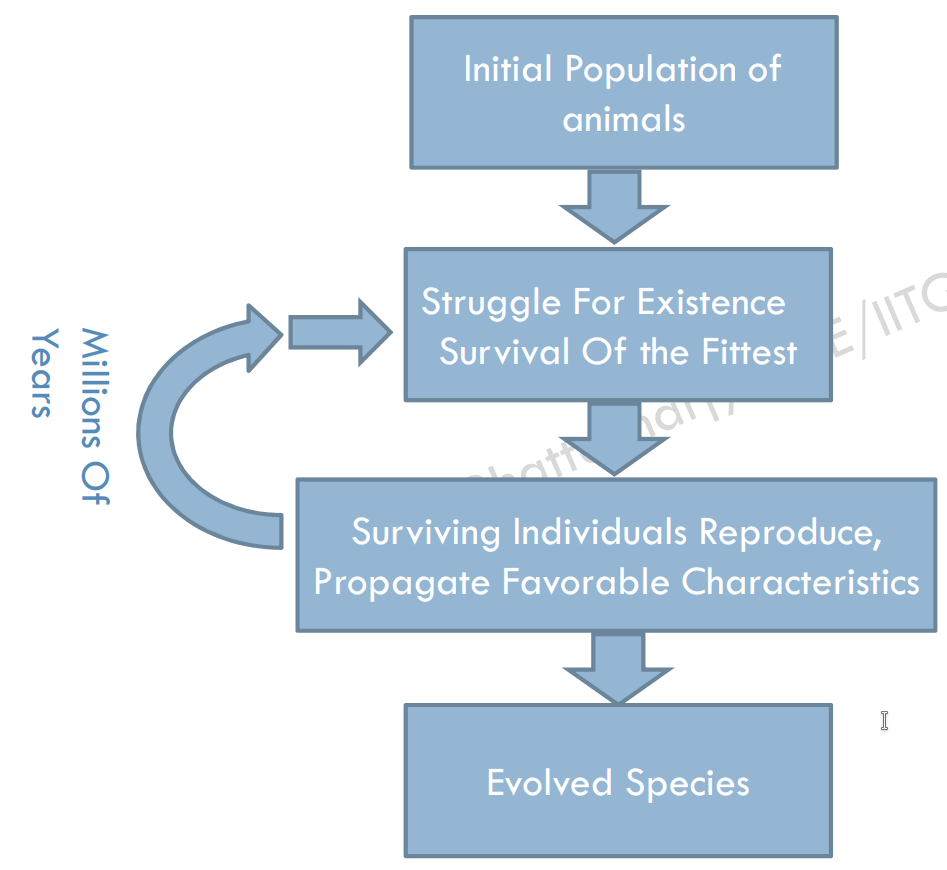
\includegraphics[width=0.7\textwidth]{img/evo2}
  \end{figure}
\end{frame}

\begin{frame}
  \frametitle{Algoritmos genético simple}
  \begin{figure}[!h] 
    \centering
    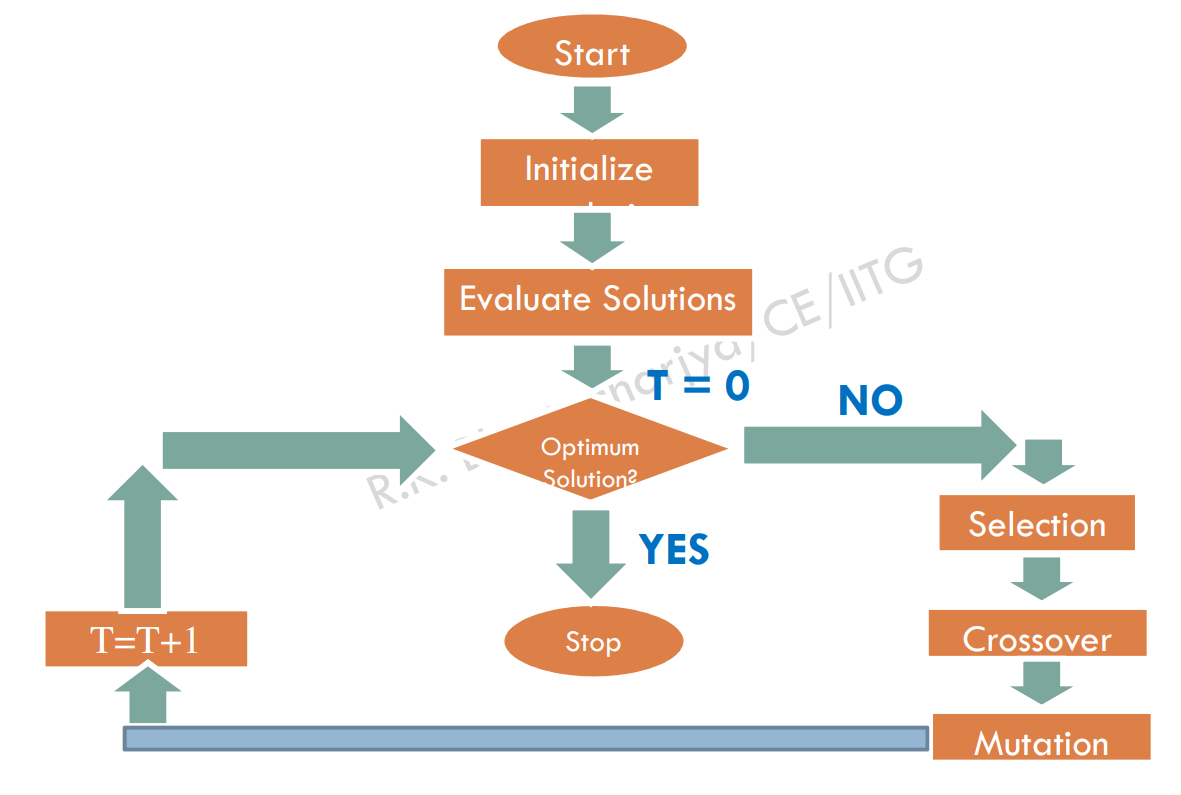
\includegraphics[width=0.9\textwidth]{img/gen1}
  \end{figure}
\end{frame}

\subsection{Operadores y parámetros}

\begin{frame}
  \frametitle{Operadores de AG}
  \begin{itemize}
    \item Selección.
    \item Cruce o \textit{Crossover}.
    \item Mutación.
  \end{itemize}
\end{frame}

\begin{frame}
  \frametitle{Selección}
  Este proceso determina cuáles soluciones se mantienen y se permiten
  reproducirse y cuáles merecen desaparecer.

  El objetivo principal del operador de selección es el de destacar soluciones 
  con buen desempeño y eliminar soluciones con mal desempeño mientras se mantiene 
  el tamaño de la población constante.

  \begin{quote}
    Selecciona al mejor, descarta al resto.
  \end{quote}
\end{frame}

\begin{frame}
  \frametitle{Selección}
  El operador de selección debe cumplir las siguientes funciones:
  \begin{itemize}
    \item Identificar soluciones ``buenas''.
    \item Hacer copias múltiples de las buenas soluciones.
    \item Eliminar soluciones malas de la población para 
    que las copias de las buenas puedan tomar su lugar.
  \end{itemize}
  \pause
  Cómo identificar las \alert{buenas soluciones}?
\end{frame}

\begin{frame}
  \frametitle{Función de competencia o Fitness function}
  \begin{itemize}
    \item Se asigna un valor de competencia o \textit{fitness} para evaluar cada solución.
    \item La función de competencia cuantifica la optimalidad de una solución.
    \item El valor es usado para rankear una solución dentro de las demás.
    \item El valor de competencia es asignado en función de su cercanía a la solución óptima al problema.
  \end{itemize}

\end{frame}

\begin{frame}
  \frametitle{Implementación del operador de Selección}
  Existen distintas técnicas para implementar la selección en AG.
  \begin{itemize}
    \item Selección por torneo.
    \item Selección por la ruleta.
    \item Selección proporcional.
    \item Selección por ranking.
    \item Selección por estado estable.
  \end{itemize}
\end{frame}

\begin{frame}
  \frametitle{Selección por torneo}

  \begin{itemize}
    \item Se realizan varios  ``torneos'' o competencias entre algunos individuos seleccionados aleatoriamente.
    \item El ganador de cada torneo es seleccionado para la siguiente generación.
    \item La rigurosidad de la selección se puede ajustar con el tamaño del torneo.
    \item Los individuos débiles tienen menor chance en torneos grandes.
  \end{itemize}

\end{frame}

\begin{frame}
  \frametitle{Selección por ruleta y proporcional}

  \begin{columns}
    \begin{column}{0.4\textwidth}
        Se ordena a los individuos y se asigna un porcentaje en la ruleta.
        Los mejores individuos tienen más chances de ser seleccionados.
    \end{column}
    \begin{column}{0.6\textwidth}
      \begin{figure}[!h] 
        \centering
        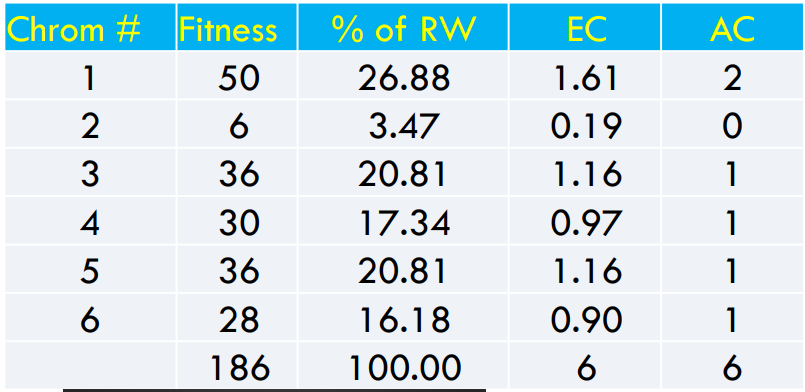
\includegraphics[width=1\textwidth]{img/ruleta1}
      \end{figure}  
    \end{column}
  \end{columns}

\end{frame}

\begin{frame}
  \frametitle{Selección por ruleta y proporcional}

  \begin{columns}
    \begin{column}{0.4\textwidth}
      \begin{figure}[!h] 
        \centering
        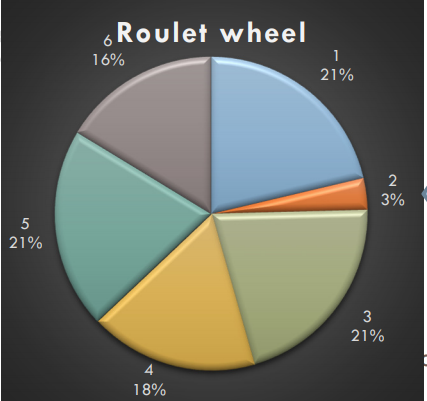
\includegraphics[width=1\textwidth]{img/ruleta2}
      \end{figure} 
    \end{column}
    \begin{column}{0.6\textwidth}
      \begin{figure}[!h] 
        \centering
        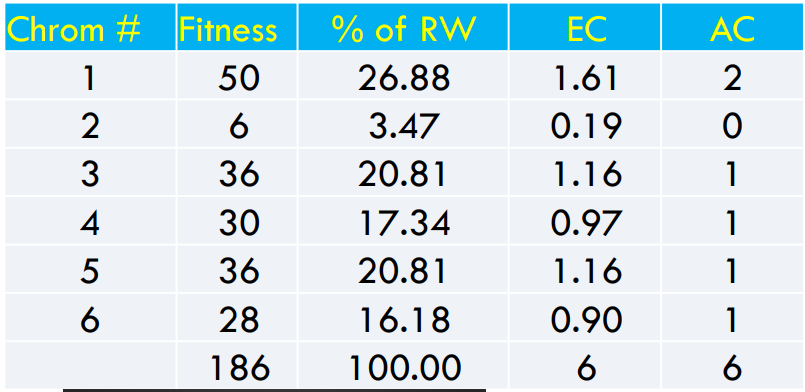
\includegraphics[width=1\textwidth]{img/ruleta1}
      \end{figure}  
    \end{column}
  \end{columns}

\end{frame}

\begin{frame}
  \frametitle{Selección por ranking}
  Se ordena a los individuos de acuerdo a su competencia y se asigna un 
  ranking. Luego se procede a definir la cantidad de copias.
  

\end{frame}


\begin{frame}
  \frametitle{Selección por ranking}
  
  \begin{figure}[!h] 
    \centering
    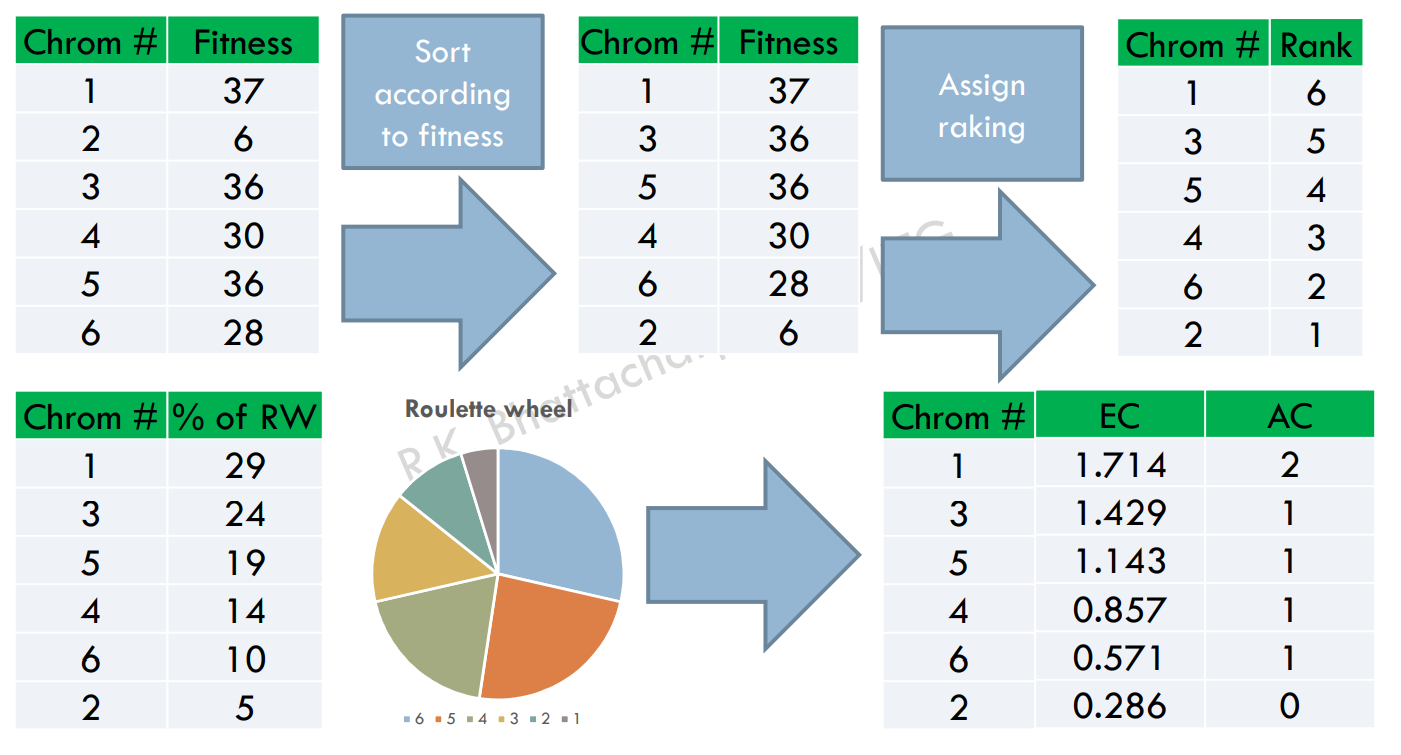
\includegraphics[width=1\textwidth]{img/rank}
  \end{figure}

\end{frame}

\begin{frame}
  \frametitle{Crossover}

  Se usa el operador de Crossover para crear nuevas soluciones en base a 
  soluciones existentes disponibles despues de aplicar el operador de selección.

  Este operador intercambia información genética entre las soluciones más fuertes.

  \begin{figure}[!h] 
    \centering
    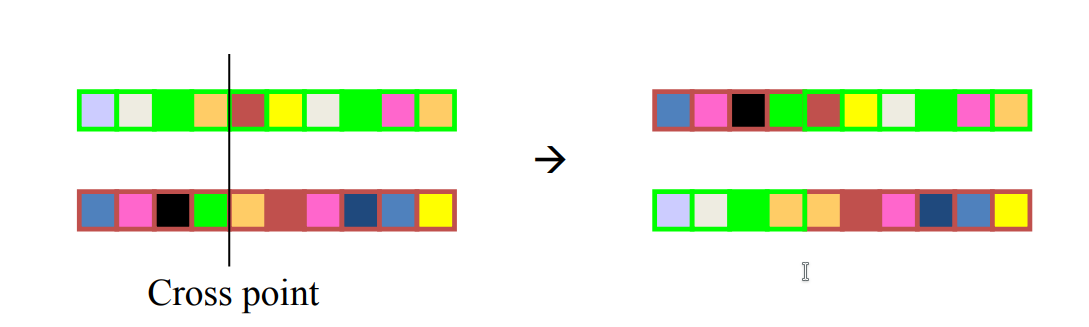
\includegraphics[width=1\textwidth]{img/cross}
  \end{figure}

  El \textit{cross point} se suele elegir de forma aleatoria.

\end{frame}

\begin{frame}
  \frametitle{Mutación}

  La mutación refiere a la introducción ocasional de nuevas características en 
  la naturaleza de las soluciones para mantener un nivel de diversidad.

  Pese a que el crossover tiene la principal responsabilidad en la búsqueda de 
  la solución óptima, la mutación también se usa con este propósito.
  \begin{figure}[!h] 
    \centering
    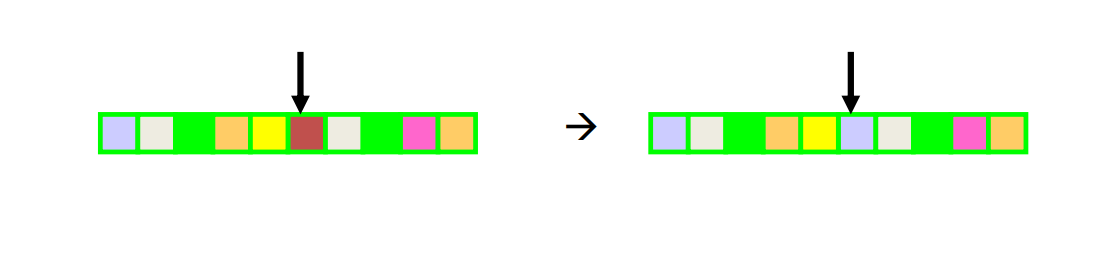
\includegraphics[width=1\textwidth]{img/mut}
  \end{figure}

\end{frame}

\begin{frame}
  \frametitle{Elitismo}

  La combinación de crossover y mutación puede eliminar a la mejor solución de 
  la población. Elitismo se define como la preservación de las mejores soluciones de 
  la población como un porcentaje de la misma.

\end{frame}

\begin{frame}
  \frametitle{Equivalencias biológicas}

  Los componentes de un AG se pueden equiparar a distintos fenónemos en la naturaleza.

  \begin{itemize}
    \item Población: Conjunto de soluciones.
    \item Individuo: Solución a un problema.
    \item Fitness: Calidad de la solución.
    \item Cromosoma: Codificación de la solución.
    \item Gen: Parte unitaria de la codificación de la solución.
  \end{itemize}

\end{frame}

\begin{frame}
  \frametitle{Ejemplo: Traveling Salesman Problem}

  En este problema se debe encontrar un recorrido en un conjunto de ciudades 
  o locaciones en el cual:
  
  \begin{itemize}
    \item cada ciudad es visitada al menos una vez.
    \item la distancia total recorrida es mínima.
  \end{itemize}

\end{frame}

\begin{frame}
  \frametitle{Representación}

  La Representación de las soluciones es una lista ordenada de ciudades representadas 
  por un número. Este tipo de representación corresponde a un Algoritmo Genético basado
  en ordenamiento.

  \begin{columns}
    \begin{column}{0.5\textwidth}
      \begin{itemize}
        \item Lista1: (3 5 7 2 1 6 4 8)
        \item Lista2: (2 5 7 6 8 1 3 4)
      \end{itemize} 
    \end{column}
    \begin{column}{0.5\textwidth}
      \begin{enumerate}
        \item La Paz
        \item Santa Cruz
        \item Oruro
        \item Potosí
        \item Cochabamba
        \item Sucre
        \item Trinidad
        \item Tarija
      \end{enumerate} 
    \end{column}
  \end{columns}

\end{frame}

\begin{frame}
  \frametitle{Crossover}

  Se combina inversión y recombinación:

  \begin{figure}[!h] 
    \centering
    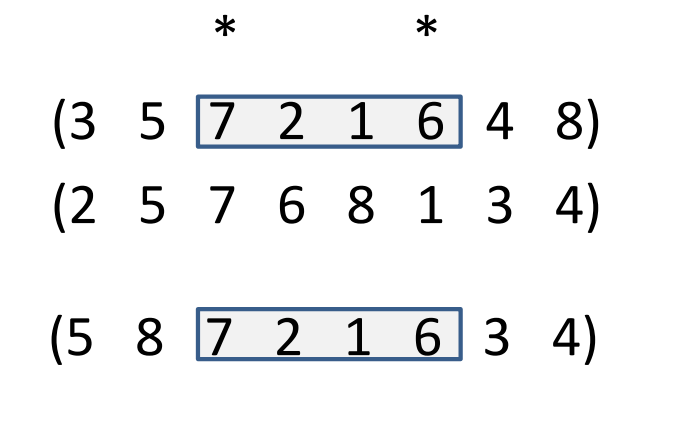
\includegraphics[width=0.6\textwidth]{img/cross2}
  \end{figure}

\end{frame}

\begin{frame}
  \frametitle{Mutación}

  La mutación consiste en un reordenamiento.

  \begin{figure}[!h] 
    \centering
    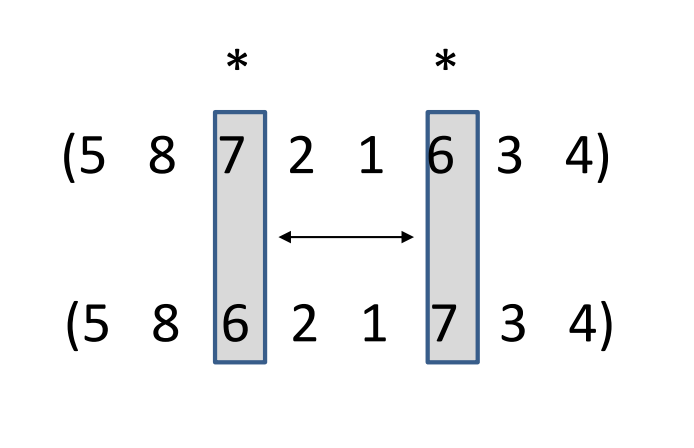
\includegraphics[width=0.6\textwidth]{img/mut2}
  \end{figure}

\end{frame}

\begin{frame}
  \frametitle{Ejemplo con 30 ciudades}

  \begin{figure}[!h] 
    \centering
    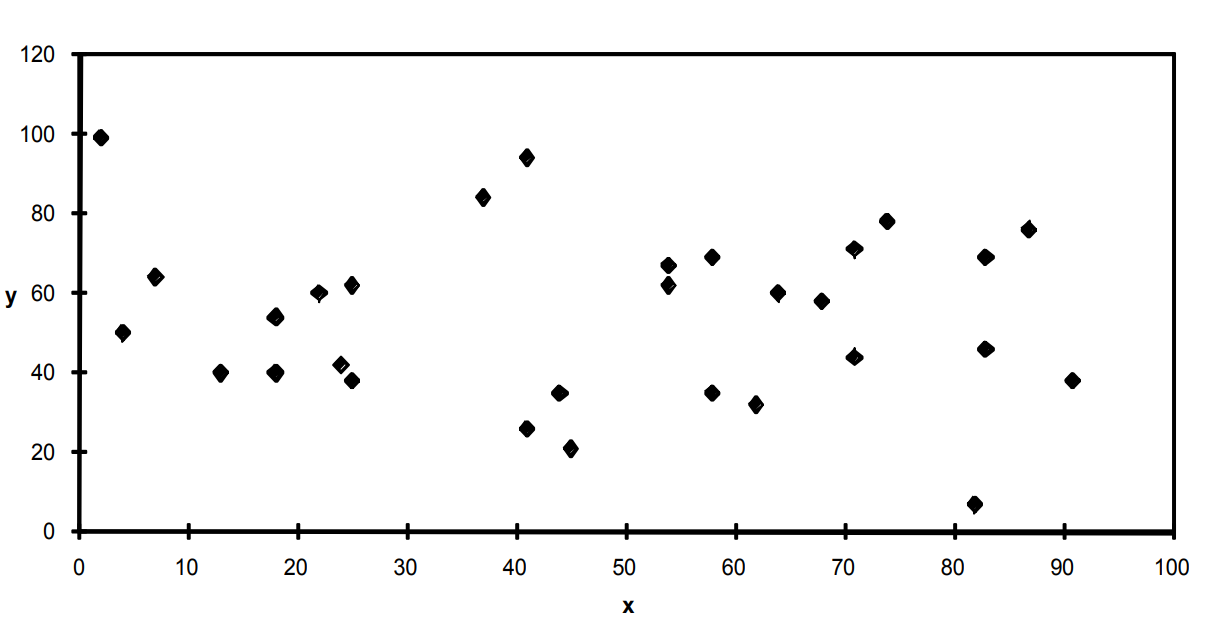
\includegraphics[width=1\textwidth]{img/tsp1}
  \end{figure}

\end{frame}

\begin{frame}
  \frametitle{Ejemplo con 30 ciudades, distancia=941}

  \begin{figure}[!h] 
    \centering
    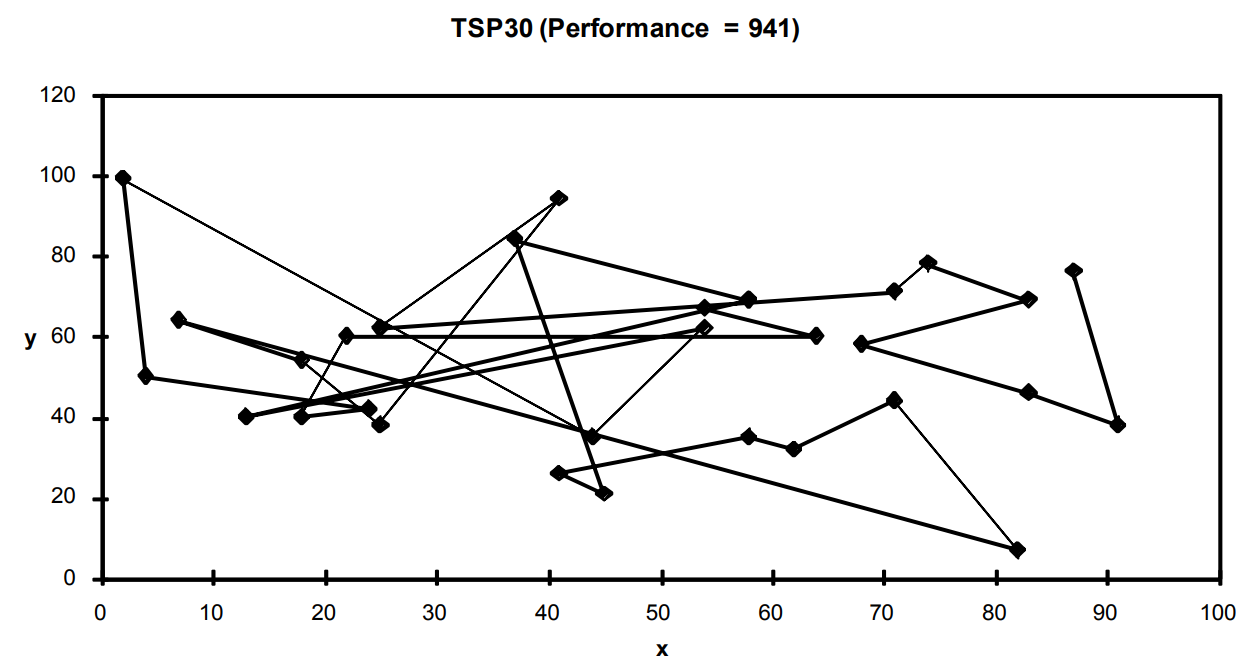
\includegraphics[width=1\textwidth]{img/tsp2}
  \end{figure}

\end{frame}

\begin{frame}
  \frametitle{Ejemplo con 30 ciudades, distancia=800}

  \begin{figure}[!h] 
    \centering
    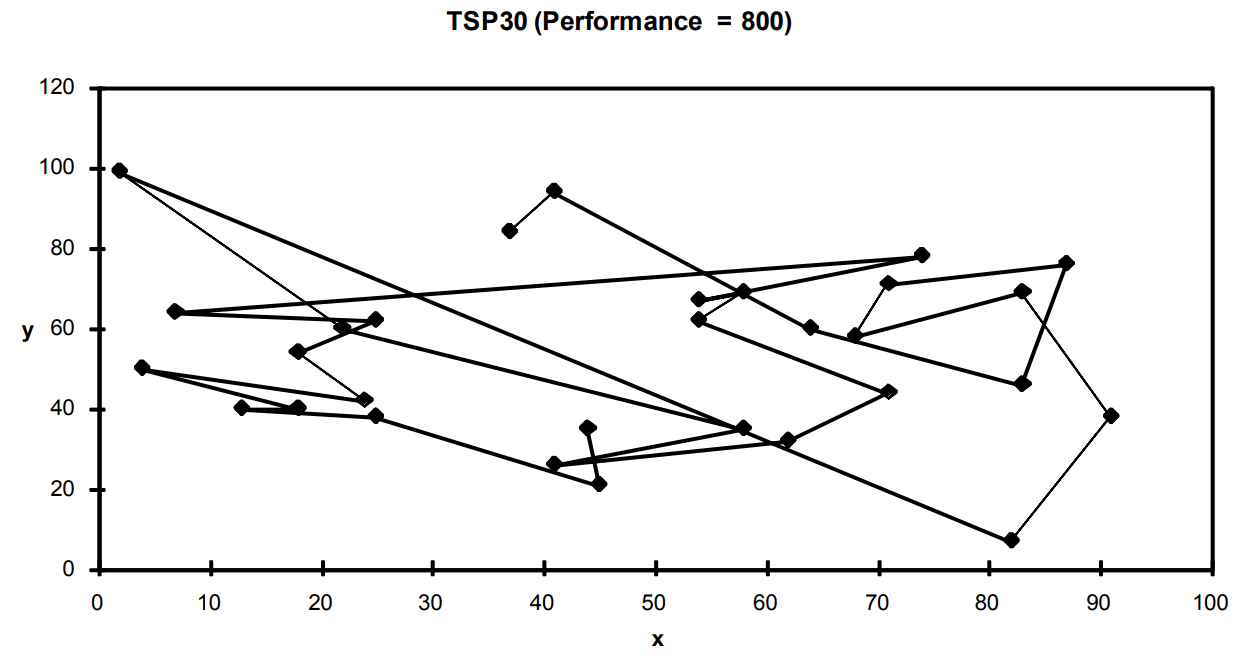
\includegraphics[width=1\textwidth]{img/tsp3}
  \end{figure}

\end{frame}

\begin{frame}
  \frametitle{Ejemplo con 30 ciudades, distancia=652}

  \begin{figure}[!h] 
    \centering
    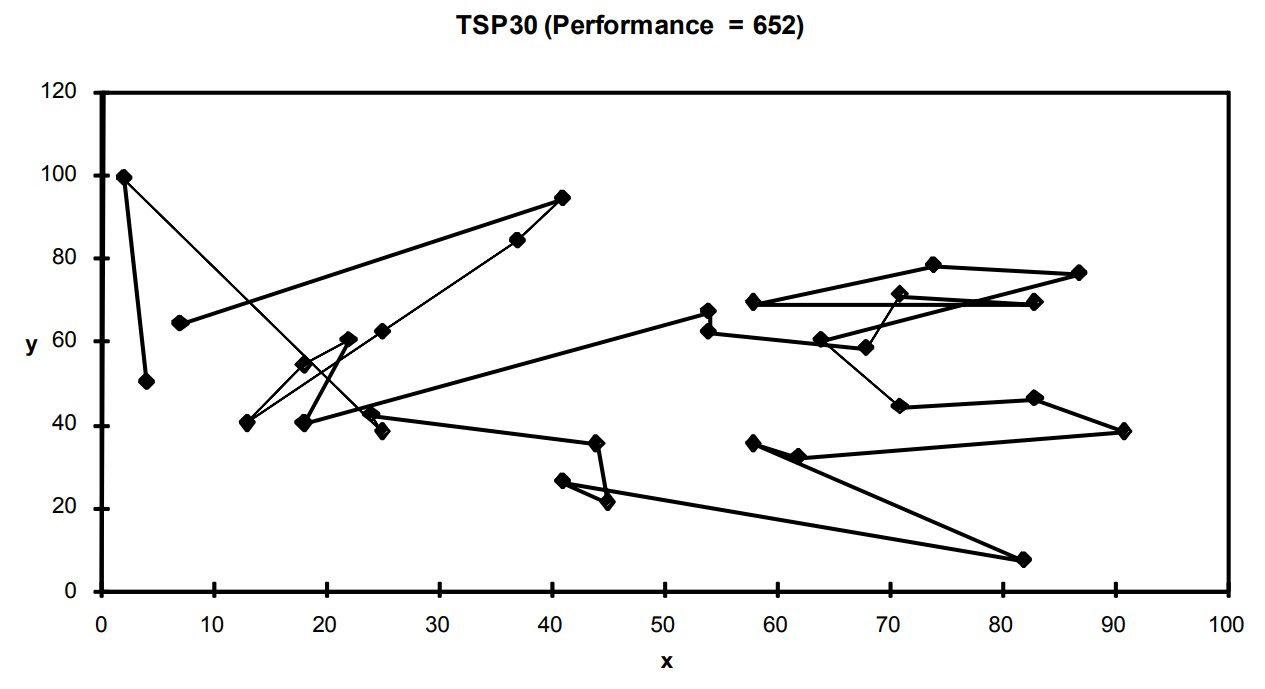
\includegraphics[width=1\textwidth]{img/tsp4}
  \end{figure}

\end{frame}

\begin{frame}
  \frametitle{Ejemplo con 30 ciudades, distancia=420}

  \begin{figure}[!h] 
    \centering
    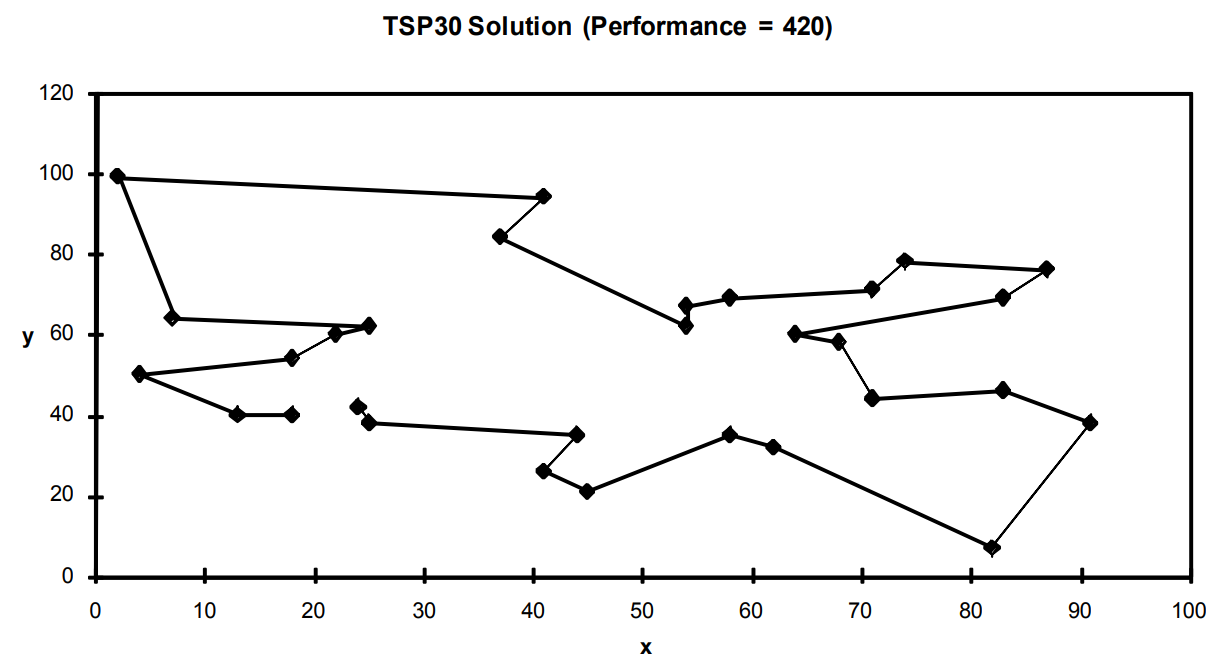
\includegraphics[width=1\textwidth]{img/tsp5}
  \end{figure}

\end{frame}


\begin{frame}
  \frametitle{Aplicaciones}

  Los AG tienen varias aplicaciones en diversas áreas:
  \begin{itemize}
    \item \textbf{Control:} Gasoductos, evasión de misiles.
    \item \textbf{Diseño:} Diseño de aeronaves, redes de comunicaciones.
    \item \textbf{Juegos:} Poker, damas, otros juegos adversarios.
    \item \textbf{Seguridad:} Encriptación.
    \item \textbf{Robótica:} Planeamiento de trayectorias.
  \end{itemize}

\end{frame}

\begin{frame}
  \frametitle{Ventajas} 

  \begin{itemize}
    \item Conceptualmente fácil de entender.
    \item Modular, independiente de la aplicación.
    \item Soporta optimización multiobjetivo.
    \item Siempre presenta una solución, y ésta mejora con el tiempo.
    \item Se puede aprovechar soluciones previas o alternativas.
    \item Flexibilidad y extensibilidad para aplicaciones híbridas (Neuroevolución).
  \end{itemize}

\end{frame}

{\setbeamercolor{palette primary}{fg=black, bg=yellow}
\begin{frame}[standout]
  Demo Time
  \begin{itemize}
    \item \href{http://math.hws.edu/eck/jsdemo/jsGeneticAlgorithm.html}{demo1}
    \item \href{https://rednuht.org/genetic_walkers/}{demo2}
    \item \href{https://rednuht.org/genetic_cars_2/}{demo3}
  \end{itemize}
\end{frame}
}

{\setbeamercolor{palette primary}{fg=black, bg=yellow}
\begin{frame}[standout]
  Preguntas?
\end{frame}
}

\appendix


\end{document}
